\section{Hardware design and Implementation}

\subsection{Module Waveform Generator}

\subsubsection{Module Sine Waveform}
\begin{figure}[H]
	\centering
	\fbox{%
		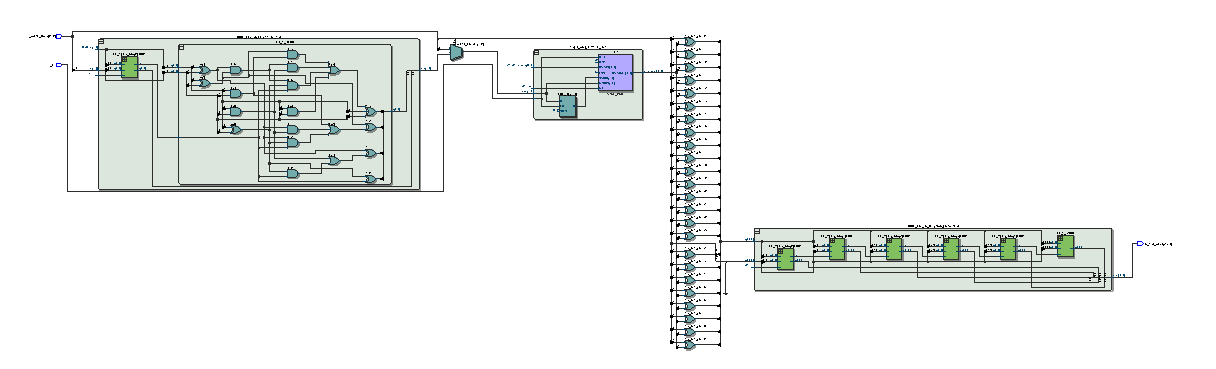
\includegraphics[width=\linewidth]{./my-chapters/my-diagrams/wave_sin.pdf}%
	}
	\caption{Block diagram for Module Sin\_Wave.}
\end{figure}

\subsubsection{Module Square Waveform}
\begin{figure}[H]
	\centering
	\fbox{%
		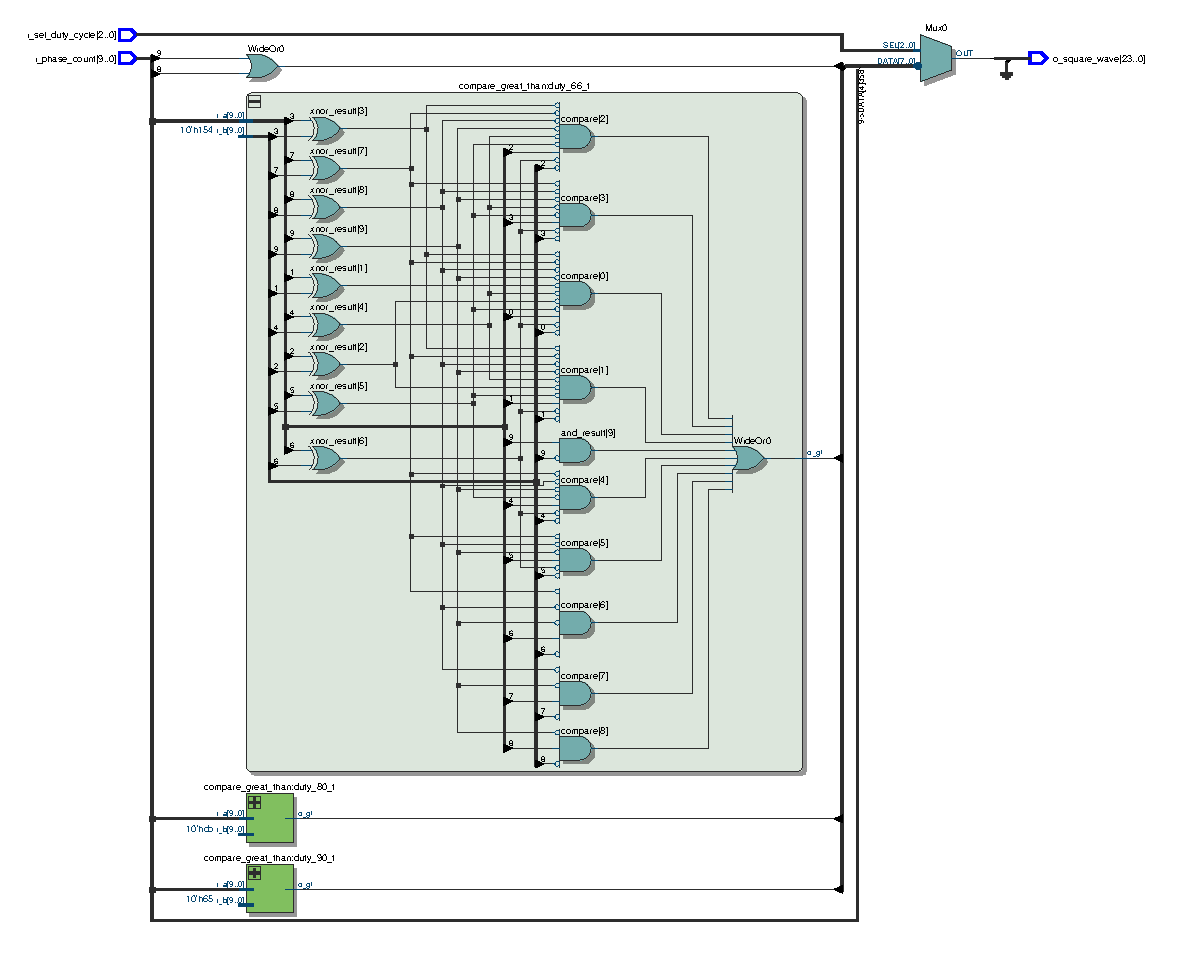
\includegraphics[width=\linewidth]{./my-chapters/my-diagrams/wave_square.pdf}%
	}
	\caption{Block diagram for Module Square\_wave.}
\end{figure}

\subsubsection{Module Triangle Waveform}
\begin{figure}[H]
	\centering
	\fbox{%
		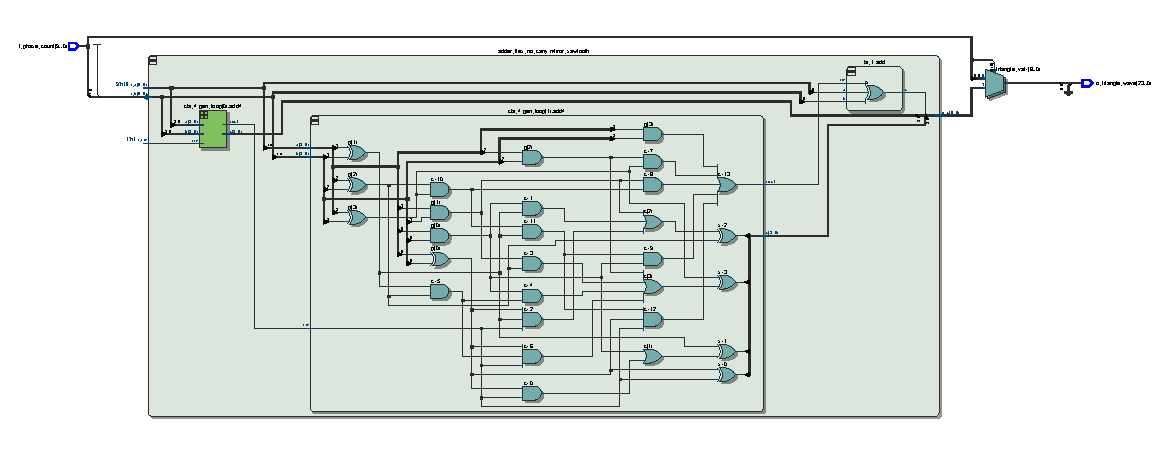
\includegraphics[width=\linewidth]{./my-chapters/my-diagrams/wave_triangle.pdf}%
	}
	\caption{Block diagram for Module Triangle\_wave.}
\end{figure}

\subsubsection{Module Sawtooth Waveform}
\begin{figure}[H]
	\centering
	\fbox{%
		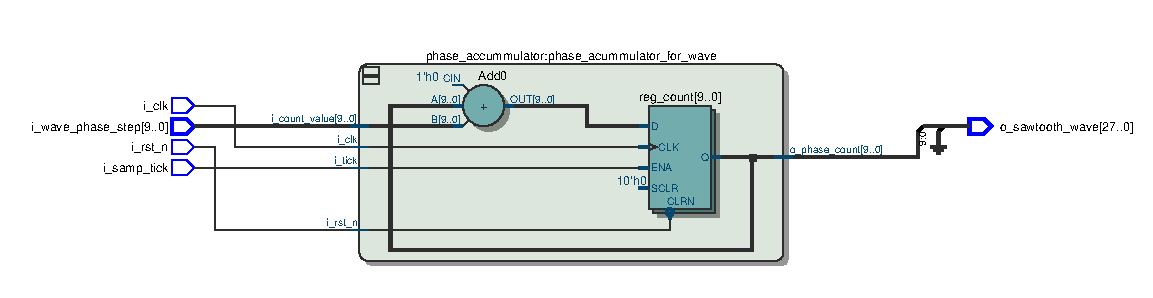
\includegraphics[width=\linewidth]{./my-chapters/my-diagrams/wave_sawtooth.pdf}%
	}
	\caption{Block diagram for Module Sawtooth\_wave.}
\end{figure}

\subsubsection{Module ECG Waveform}
\begin{figure}[H]
	\centering
	\fbox{%
		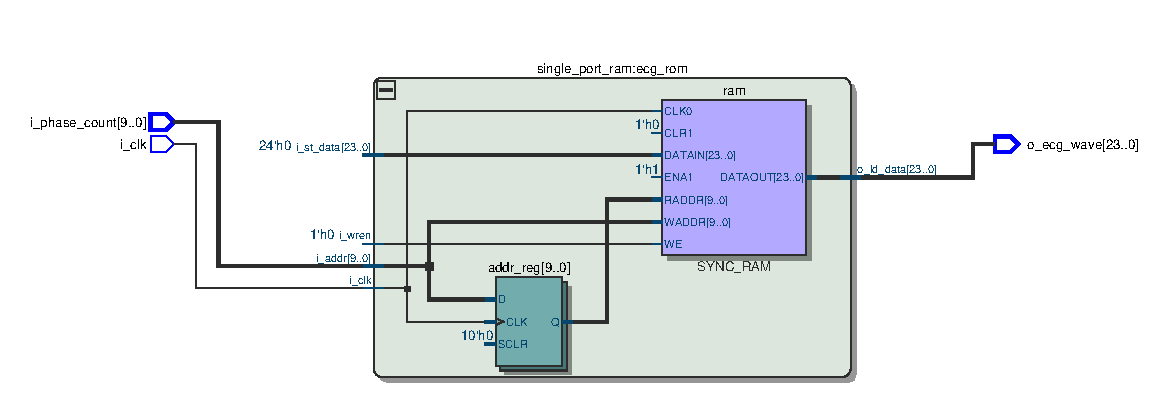
\includegraphics[width=\linewidth]{./my-chapters/my-diagrams/wave_ecg.pdf}%
	}
	\caption{Block diagram for Module ECG\_wave.}
\end{figure}

\subsubsection{Module Waveform Generator}
\begin{figure}[H]
	\centering
	\fbox{%
		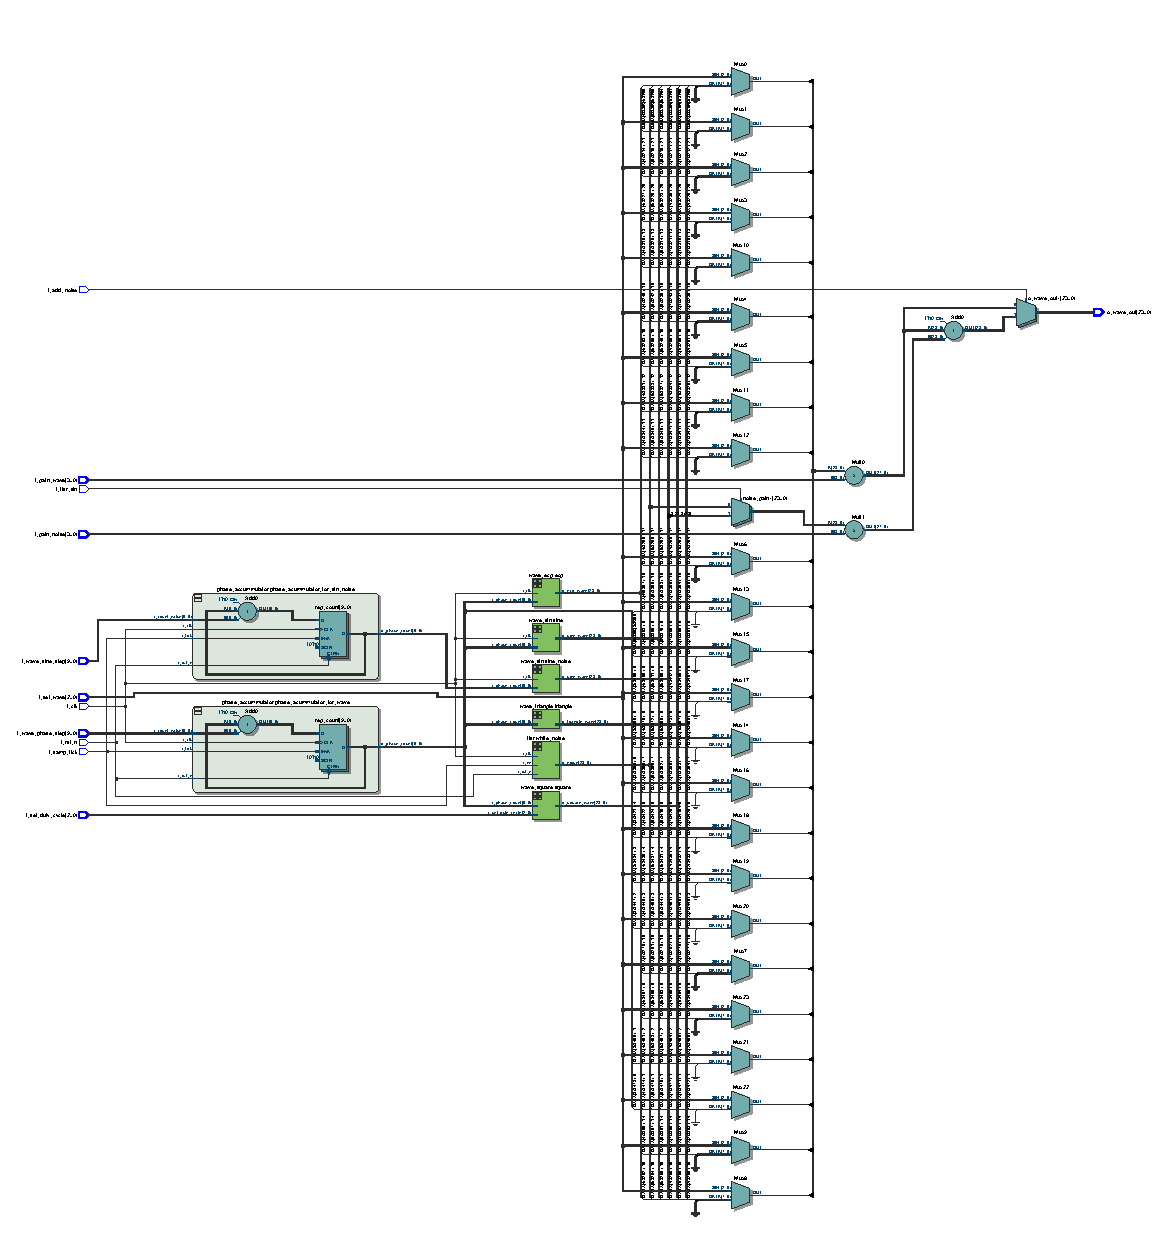
\includegraphics[width=\linewidth]{./my-chapters/my-diagrams/wave_gen.pdf}%
	}
	\caption{Block diagram for Module Waveform Generator.}
\end{figure}

\subsection{Module Control value}

\begin{figure}[H]
	\centering
	\includegraphics[width=.8\linewidth, height=0.7\textheight]{./../00_spec/spec/UI_task.png}
	\caption{Communication operations between the user and the Control Value Module.}
\end{figure}

\begin{figure}[H]
	\centering
	\includegraphics[width=.8\linewidth]{./../00_spec/spec/UI_rtl.png}
	\caption{Block diagram for Module Control value.}
\end{figure}

